\documentclass[11pt,twocolumn]{article}

% ─── Packages ─────────────────────────────────────────────────────
\usepackage[T1]{fontenc}
\usepackage[utf8]{inputenc}
\usepackage{lmodern}
\usepackage[margin=0.85in,top=1in,bottom=1in]{geometry}
\usepackage{graphicx}
\usepackage{xcolor}
\usepackage{tikz}
\usetikzlibrary{positioning,arrows.meta,fit,shapes.geometric,calc,
                decorations.pathreplacing,backgrounds,matrix}
\usepackage{booktabs}
\usepackage{enumitem}
\usepackage{listings}
\usepackage{hyperref}
\usepackage{amsmath,amssymb}
\usepackage{caption}
\usepackage{subcaption}
\usepackage{fancyhdr}
\usepackage{titlesec}
\usepackage{abstract}
\usepackage{float}
\usepackage{tabularx}

% ─── Colors ───────────────────────────────────────────────────────
\definecolor{dom0blue}{HTML}{3874D8}
\definecolor{vmorange}{HTML}{E38B28}
\definecolor{keygreen}{HTML}{3FB950}
\definecolor{hmacpurple}{HTML}{8957E5}
\definecolor{dangerred}{HTML}{DA3633}
\definecolor{codebg}{HTML}{161B22}
\definecolor{codefg}{HTML}{C9D1D9}
\definecolor{codegreen}{HTML}{7EE787}
\definecolor{codeblue}{HTML}{79C0FF}
\definecolor{accentblue}{HTML}{58A6FF}
\definecolor{auditgold}{HTML}{D29922}
\definecolor{queuecyan}{HTML}{39D2C0}

% ─── Listings ─────────────────────────────────────────────────────
\lstdefinestyle{terminal}{
    backgroundcolor=\color{codebg},
    basicstyle=\ttfamily\scriptsize\color{codefg},
    keywordstyle=\color{codeblue},
    stringstyle=\color{codegreen},
    commentstyle=\color{gray},
    frame=single,
    rulecolor=\color{gray!30},
    breaklines=true,
    columns=fullflexible,
    xleftmargin=4pt,
    xrightmargin=4pt,
    aboveskip=8pt,
    belowskip=8pt,
}

\lstdefinestyle{python}{
    backgroundcolor=\color{codebg},
    basicstyle=\ttfamily\scriptsize\color{codefg},
    keywordstyle=\color{codeblue}\bfseries,
    stringstyle=\color{codegreen},
    commentstyle=\color{gray}\itshape,
    frame=single,
    rulecolor=\color{gray!30},
    breaklines=true,
    columns=fullflexible,
    xleftmargin=4pt,
    xrightmargin=4pt,
    aboveskip=8pt,
    belowskip=8pt,
    language=Python,
    morekeywords={hmac,hashlib,secrets,subprocess,Path},
}

% ─── Hyperref ─────────────────────────────────────────────────────
\hypersetup{
    colorlinks=true,
    linkcolor=dom0blue,
    citecolor=dom0blue,
    urlcolor=accentblue,
}

% ─── Headers ──────────────────────────────────────────────────────
\pagestyle{fancy}
\fancyhf{}
\fancyhead[L]{\small\textit{qvm-remote: Reverse Shell for Qubes OS dom0}}
\fancyhead[R]{\small\thepage}
\renewcommand{\headrulewidth}{0.4pt}

% ─── Title ────────────────────────────────────────────────────────
\title{%
    \vspace{-1em}%
    \textbf{\Large qvm-remote: Authenticated Remote Execution\\in Qubes OS dom0 via File-Based Queues}\\[6pt]
    \large A Pull-Model RPC Framework with HMAC-SHA256\\Authentication and Full Audit Trails%
}

\author{%
    Gabriele Risso\\
    \texttt{gabri.risso@gmail.com}\\
    \url{https://github.com/GabrieleRisso/qvm-remote}
}

\date{February 2026}

% ══════════════════════════════════════════════════════════════════
\begin{document}
\maketitle
\thispagestyle{fancy}

% ─── Abstract ─────────────────────────────────────────────────────
\begin{abstract}
\noindent
Qubes OS enforces strict isolation by prohibiting code execution from
virtual machines (VMs) in the privileged \texttt{dom0} domain. While
essential for security, this restriction creates significant friction for
developers, system administrators, and automation pipelines that need to
manage VMs programmatically. We present \textbf{qvm-remote}, an
open-source tool that provides ``SSH for dom0''---authenticated remote
command execution from VMs to \texttt{dom0} through a file-based queue
protocol. The system uses a pull model where \texttt{dom0} initiates all
I/O (never the VM), HMAC-SHA256 authentication with 256-bit per-VM keys,
comprehensive input validation, and dual-sided audit logging. We describe
the protocol design, analyze its security properties against the Qubes
threat model, present a formal analysis of the authentication scheme, and
demonstrate that the framework adds $<$50\,ms overhead per command while
providing cryptographic guarantees against replay, forgery, and
cross-VM attacks. qvm-remote is implemented in pure Python~3 (stdlib
only) and is packaged for Fedora RPM, Arch Linux, and the Qubes Builder
v2 build system.

\medskip
\noindent\textbf{Keywords:} Qubes OS, dom0, remote execution, HMAC-SHA256,
file-based queue, pull model, qrexec, system administration, Xen
\end{abstract}

% ─── 1. Introduction ─────────────────────────────────────────────
\section{Introduction}
\label{sec:intro}

Qubes OS~\cite{rutkowska2010qubes} implements a
security-by-compartmentalization architecture where the privileged
\texttt{dom0} domain manages all VMs but is intentionally isolated from
them. This design prevents a compromised VM from executing code in
\texttt{dom0}---a critical security property, since \texttt{dom0} has
unrestricted access to all VM memory, storage, and configuration.

However, this same property creates a significant usability barrier for
legitimate administration tasks. Consider a developer working in a
\texttt{code} VM who needs to:

\begin{itemize}[leftmargin=*,topsep=2pt,itemsep=1pt]
    \item Resize another VM's memory: \texttt{qvm-prefs work memory 4096}
    \item List running VMs: \texttt{qvm-ls --running}
    \item Deploy a service: \texttt{systemctl start my-tunnel}
    \item Query hypervisor state: \texttt{xl info}
\end{itemize}

Each of these requires physically switching to the \texttt{dom0}
terminal, typing the command, and switching back---a context switch that
breaks flow and discourages automation.

\textbf{qvm-remote} bridges this gap with a carefully designed protocol
that provides VM-to-dom0 command execution while preserving auditability
and cryptographic authentication. The key design principle is the
\textit{pull model}: \texttt{dom0} always initiates I/O operations,
never the VM. The VM merely writes requests to its own local filesystem;
\texttt{dom0} discovers and processes them at its own pace.

\subsection{Contributions}

\begin{itemize}[leftmargin=*,topsep=2pt,itemsep=1pt]
    \item A \textbf{file-based queue protocol} for VM-to-dom0 RPC that
          preserves the pull-model invariant
          (Section~\ref{sec:protocol}).
    \item An \textbf{HMAC-SHA256 authentication scheme} with per-VM keys
          and per-command tokens that prevents forgery, replay, and
          cross-VM attacks (Section~\ref{sec:auth}).
    \item A \textbf{defense-in-depth security model} with input
          validation, execution sandboxing, and dual-sided audit trails
          (Section~\ref{sec:security}).
    \item A \textbf{production implementation} in pure Python~3 with
          zero external dependencies, packaged for RPM, Arch, Salt, and
          Qubes Builder (Section~\ref{sec:impl}).
\end{itemize}

% ─── 2. Background ───────────────────────────────────────────────
\section{Background and Motivation}
\label{sec:background}

\subsection{The dom0 Isolation Principle}

In the Qubes security model, \texttt{dom0}:

\begin{enumerate}[leftmargin=*,topsep=2pt,itemsep=1pt]
    \item Has \textbf{no network interface}---immune to remote attack.
    \item Runs the \textbf{Xen toolstack} (\texttt{xl}, \texttt{libvirt}).
    \item Hosts the \textbf{GUI compositor} (rendering VM windows).
    \item Manages \textbf{qrexec policies}---the inter-VM firewall.
\end{enumerate}

\noindent Any code executing in \texttt{dom0} runs with the privilege
level of the hypervisor management plane. This is why Qubes treats
\texttt{dom0} as sacrosanct: no VM should be able to cause code
execution there.

\subsection{Existing Approaches}

\begin{description}[leftmargin=0pt,topsep=4pt,itemsep=2pt]
    \item[Manual switching:] The default. Secure but disruptive to
        workflow. Incompatible with automation.
    \item[Custom qrexec services:] Each command requires a separate
        \texttt{/etc/qubes-rpc/} handler and policy. Scales poorly for
        ad-hoc commands.
    \item[qubes-remote (v0.x):] An earlier bash-based prototype by the
        same author. Limited error handling, no HMAC auth, no audit
        trail, no input validation.
\end{description}

qvm-remote addresses all of these limitations with a unified, authenticated,
and auditable framework.

% ─── 3. Protocol Design ──────────────────────────────────────────
\section{Protocol Design}
\label{sec:protocol}

% ─── Protocol Diagram ────────────────────────────────────────────
\begin{figure*}[t]
\centering
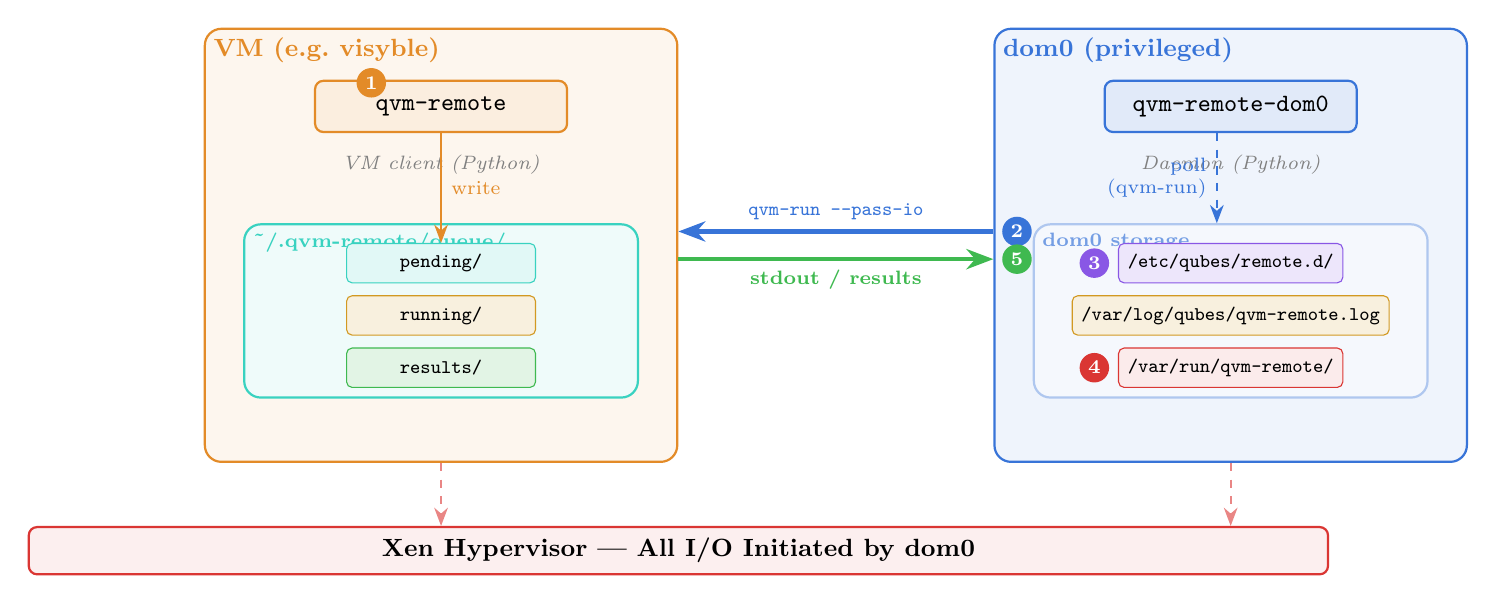
\begin{tikzpicture}[
    >=Stealth,
    node distance=0.4cm,
    box/.style={draw, rounded corners=3pt, minimum width=3.2cm,
                minimum height=0.65cm, font=\small\ttfamily, thick},
    qbox/.style={draw, rounded corners=2pt, minimum width=2.4cm,
                 minimum height=0.5cm, font=\scriptsize\ttfamily},
    dombox/.style={draw, rounded corners=6pt, thick, inner sep=10pt},
    arrow/.style={->, thick, >=Stealth},
    darrow/.style={<->, thick, >=Stealth},
    label/.style={font=\small\bfseries, anchor=north west},
]

% VM domain
\node[dombox, fill=vmorange!8, draw=vmorange, minimum width=6cm,
      minimum height=5.5cm] (vmdom) at (0,0) {};
\node[label, color=vmorange] at (vmdom.north west) {VM (e.g.\ visyble)};
\node[box, fill=vmorange!15, draw=vmorange] (client)
    at ([yshift=-1cm]vmdom.north) {qvm-remote};
\node[font=\scriptsize\itshape, color=gray, below=0.15cm of client]
    (clabel) {VM client (Python)};

% Queue structure
\node[dombox, fill=queuecyan!8, draw=queuecyan, minimum width=5cm,
      minimum height=2.2cm, below=0.5cm of clabel] (queue) {};
\node[label, color=queuecyan, font=\scriptsize\bfseries]
    at (queue.north west) {\textasciitilde/.qvm-remote/queue/};
\node[qbox, fill=queuecyan!15, draw=queuecyan, below=0.25cm of queue.north]
    (pending) {pending/};
\node[qbox, fill=auditgold!15, draw=auditgold, below=0.15cm of pending]
    (running) {running/};
\node[qbox, fill=keygreen!15, draw=keygreen, below=0.15cm of running]
    (results) {results/};

% dom0 domain
\node[dombox, fill=dom0blue!8, draw=dom0blue, minimum width=6cm,
      minimum height=5.5cm, right=4cm of vmdom] (dom0dom) {};
\node[label, color=dom0blue] at (dom0dom.north west) {dom0 (privileged)};
\node[box, fill=dom0blue!15, draw=dom0blue] (daemon)
    at ([yshift=-1cm]dom0dom.north) {qvm-remote-dom0};
\node[font=\scriptsize\itshape, color=gray, below=0.15cm of daemon]
    (dlabel) {Daemon (Python)};

% Dom0 internals
\node[dombox, fill=dom0blue!5, draw=dom0blue!40, minimum width=5cm,
      minimum height=2.2cm, below=0.5cm of dlabel] (dom0int) {};
\node[label, color=dom0blue!70, font=\scriptsize\bfseries]
    at (dom0int.north west) {dom0 storage};
\node[qbox, fill=hmacpurple!15, draw=hmacpurple, below=0.25cm of dom0int.north]
    (keys) {/etc/qubes/remote.d/};
\node[qbox, fill=auditgold!15, draw=auditgold, below=0.15cm of keys]
    (log) {/var/log/qubes/qvm-remote.log};
\node[qbox, fill=dangerred!10, draw=dangerred, below=0.15cm of log]
    (workdir) {/var/run/qvm-remote/};

% Data flow arrows
\draw[arrow, color=vmorange, thick]
    (client.south) -- node[right, font=\scriptsize, color=vmorange]
    {write} (pending.north -| client.south);

\draw[arrow, color=dom0blue, thick, dashed]
    ([xshift=-5pt]daemon.south) --
    node[left, font=\scriptsize, color=dom0blue, align=right]
    {poll\\(qvm-run)} ([xshift=-5pt]dlabel.south |- dom0int.north);

% qvm-run arrows between domains
\draw[arrow, color=dom0blue, line width=1.5pt]
    ([yshift=5pt]dom0dom.west) --
    node[above, font=\scriptsize\bfseries, color=dom0blue]
    {\texttt{qvm-run --pass-io}}
    ([yshift=5pt]vmdom.east);
\draw[arrow, color=keygreen, line width=1.5pt]
    ([yshift=-5pt]vmdom.east) --
    node[below, font=\scriptsize\bfseries, color=keygreen]
    {stdout / results}
    ([yshift=-5pt]dom0dom.west);

% Step labels
\node[fill=vmorange, circle, text=white, font=\scriptsize\bfseries,
      inner sep=1.5pt] at ([xshift=-2.5cm, yshift=0.3cm]client.east) {1};
\node[fill=dom0blue, circle, text=white, font=\scriptsize\bfseries,
      inner sep=1.5pt] at ([xshift=0.3cm, yshift=5pt]dom0dom.west) {2};
\node[fill=hmacpurple, circle, text=white, font=\scriptsize\bfseries,
      inner sep=1.5pt] at ([xshift=-0.3cm]keys.west) {3};
\node[fill=dangerred, circle, text=white, font=\scriptsize\bfseries,
      inner sep=1.5pt] at ([xshift=-0.3cm]workdir.west) {4};
\node[fill=keygreen, circle, text=white, font=\scriptsize\bfseries,
      inner sep=1.5pt] at ([xshift=0.3cm, yshift=-5pt]dom0dom.west) {5};

% Xen bar
\node[draw, thick, fill=dangerred!8, draw=dangerred, rounded corners=3pt,
      minimum width=16.5cm, minimum height=0.6cm, font=\small\bfseries,
      below=0.8cm of dom0dom.south -| vmdom.east] (xen)
    {Xen Hypervisor --- All I/O Initiated by dom0};

% Connect to Xen
\draw[arrow, color=dangerred!60, dashed] (vmdom.south) -- (xen.north -| vmdom.south);
\draw[arrow, color=dangerred!60, dashed] (dom0dom.south) -- (xen.north -| dom0dom.south);

\end{tikzpicture}
\caption{qvm-remote protocol architecture.
\textbf{(1)}~VM writes command + HMAC to \texttt{pending/}.
\textbf{(2)}~dom0 polls via \texttt{qvm-run --pass-io}.
\textbf{(3)}~Verifies HMAC against stored key.
\textbf{(4)}~Executes in sandboxed work directory.
\textbf{(5)}~Writes results back to VM.
All I/O is initiated by dom0 (pull model).}
\label{fig:protocol}
\end{figure*}

% (circled command moved to preamble)

\subsection{The Pull-Model Invariant}

The fundamental design constraint is:

\begin{quote}
\textit{dom0 initiates every I/O operation. The VM never pushes data to
dom0; it only writes to its own local filesystem.}
\end{quote}

This preserves the Qubes principle that VMs cannot cause effects in
\texttt{dom0}---\texttt{dom0} \textit{chooses} to read from the VM.
The distinction is subtle but important: the VM's ``request'' is a
passive file on its own disk, not an active network connection or
syscall into \texttt{dom0}.

\subsection{Queue Structure}

Each authorized VM maintains a queue directory:

\begin{lstlisting}[style=terminal]
~/.qvm-remote/
  queue/
    pending/          # new commands
      20260218-143022-1234-a1b2c3d4
      20260218-143022-1234-a1b2c3d4.auth
    running/          # in-progress (moved by dom0)
    results/          # completed
      <cmd_id>.out    # stdout
      <cmd_id>.err    # stderr
      <cmd_id>.exit   # exit code
      <cmd_id>.meta   # timing metadata
  auth.key            # 256-bit HMAC key (0600)
  audit.log           # VM-side audit trail
  history/            # archived results
    2026-02-18/
      <cmd_id>/
\end{lstlisting}

\subsection{Command Lifecycle}

The protocol proceeds in five phases:

\begin{enumerate}[leftmargin=*,topsep=2pt,itemsep=2pt]
    \item \textbf{Enqueue} (VM): The client generates a unique command ID
          ($\mathit{cid} = \text{timestamp-pid-}\text{random}_8$),
          writes the command body to \texttt{pending/\textit{cid}}, and
          writes $\text{HMAC-SHA256}(k, \mathit{cid})$ to
          \texttt{pending/\textit{cid}.auth}.
    \item \textbf{Poll} (dom0): The daemon lists
          \texttt{pending/} via \texttt{qvm-run --pass-io --no-autostart}.
    \item \textbf{Authenticate} (dom0): For each command, reads
          \texttt{.auth}, recomputes HMAC, verifies with
          \texttt{hmac.compare\_digest}. Rejects on mismatch.
    \item \textbf{Execute} (dom0): Writes command to a 0700 work file,
          moves \textit{cid} from \texttt{pending/} to \texttt{running/},
          executes with \texttt{bash} under a timeout.
    \item \textbf{Return} (dom0): Writes \texttt{.out}, \texttt{.err},
          \texttt{.exit}, \texttt{.meta} to \texttt{results/},
          removes from \texttt{running/}, appends to audit log.
\end{enumerate}

% ─── Command ID Diagram ──────────────────────────────────────────
\begin{figure}[h]
\centering
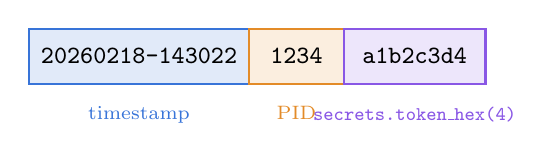
\begin{tikzpicture}[
    part/.style={draw, thick, minimum height=0.7cm, font=\small\ttfamily,
                 inner xsep=4pt},
]
\node[part, fill=dom0blue!15, draw=dom0blue, minimum width=2.8cm]
    (ts) at (0,0) {20260218-143022};
\node[part, fill=vmorange!15, draw=vmorange, minimum width=1.2cm,
      right=-\pgflinewidth of ts] (pid) {1234};
\node[part, fill=hmacpurple!15, draw=hmacpurple, minimum width=1.8cm,
      right=-\pgflinewidth of pid] (rand) {a1b2c3d4};

\node[font=\scriptsize, color=dom0blue, below=0.15cm of ts] {timestamp};
\node[font=\scriptsize, color=vmorange, below=0.15cm of pid] {PID};
\node[font=\scriptsize, color=hmacpurple, below=0.15cm of rand]
    {\texttt{secrets.token\_hex(4)}};
\end{tikzpicture}
\caption{Command ID structure. Combines wall-clock time, process ID, and
cryptographic randomness for uniqueness and non-replayability.}
\label{fig:cmdid}
\end{figure}

\subsection{The ``No Auto-Start'' Property}

A critical detail: the daemon uses \texttt{qvm-run --no-autostart}.
If an authorized VM is powered off, it is silently skipped. The daemon
never starts a VM as a side effect of polling---this prevents a
compromised configuration file from causing VM launches.

% ─── 4. Authentication ───────────────────────────────────────────
\section{Authentication Scheme}
\label{sec:auth}

\subsection{Key Management}

Each VM-dom0 pair shares a 256-bit symmetric key $k$:

\begin{itemize}[leftmargin=*,topsep=2pt,itemsep=1pt]
    \item \textbf{VM}: \texttt{\textasciitilde/.qvm-remote/auth.key}
          (mode 0600). Generated with \texttt{secrets.token\_hex(32)}.
    \item \textbf{dom0}: \texttt{/etc/qubes/remote.d/\textit{vm}.key}
          (mode 0600, directory 0700).
\end{itemize}

\noindent Key exchange is out-of-band: the user runs \texttt{qvm-remote key gen}
in the VM, then copies the key to dom0 via \texttt{qvm-remote-dom0 authorize}.
The key itself never traverses the queue protocol.

\subsection{Per-Command Tokens}

For each command with identifier $\mathit{cid}$, the VM computes:

\begin{equation}
    \tau = \text{HMAC-SHA256}(k, \mathit{cid})
\end{equation}

\noindent and writes $\tau$ (as a hex string) to
\texttt{pending/\textit{cid}.auth}. dom0 recomputes $\tau'$ from the
stored key and verifies:

\begin{equation}
    \text{valid} \iff \texttt{hmac.compare\_digest}(\tau, \tau')
\end{equation}

\noindent using Python's constant-time comparison to prevent timing
side-channel attacks.

\subsection{Security Properties}

\begin{table}[h]
\centering
\caption{Authentication properties and their guarantees.}
\label{tab:auth}
\small
\begin{tabular}{@{}p{2cm}p{4.8cm}@{}}
\toprule
\textbf{Property} & \textbf{Guarantee} \\
\midrule
Forgery resistance &
    $\Pr[\text{forge}] \leq 2^{-256}$ per attempt. Key is
    never transmitted; only HMAC tokens appear in the queue. \\
Replay resistance &
    Each $\mathit{cid}$ includes cryptographic randomness
    (\texttt{secrets.token\_hex(4)}) and a timestamp. dom0
    processes and deletes each $\mathit{cid}$ exactly once. \\
Cross-VM isolation &
    Per-VM keys. Compromising VM $A$'s key yields
    $\Pr[\text{forge}_B] = 2^{-256}$ for VM $B$. \\
Timing resistance &
    \texttt{hmac.compare\_digest} runs in constant time
    regardless of input. \\
\bottomrule
\end{tabular}
\end{table}

\subsection{Brute-Force Analysis}

The key space is $2^{256}$. At $10^{12}$ HMAC computations per second
(exceeding any current hardware), exhaustive search requires:

\begin{equation}
    \frac{2^{256}}{10^{12} \times 365.25 \times 86400}
    \approx 3.7 \times 10^{57} \text{ years}
\end{equation}

\noindent No retry limiting or lockout is needed---the key space makes
brute force mathematically irrelevant.

% ─── 5. Security Analysis ────────────────────────────────────────
\section{Security Analysis}
\label{sec:security}

qvm-remote deliberately weakens the Qubes isolation model by granting
VMs the ability to execute commands in dom0. This section analyzes the
resulting attack surface and mitigations.

% ─── Security Layers Diagram ─────────────────────────────────────
\begin{figure}[h]
\centering
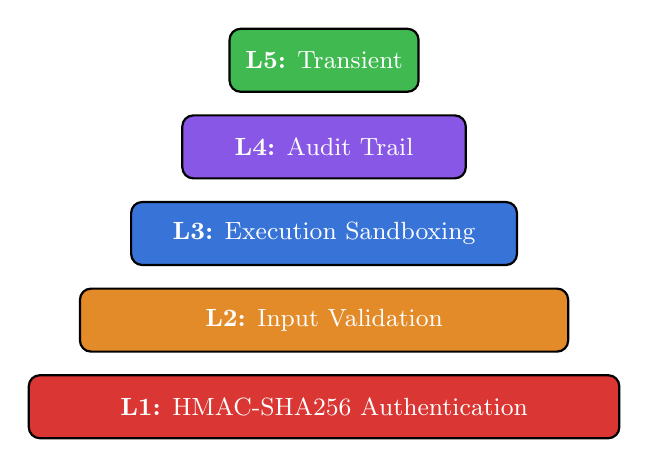
\begin{tikzpicture}[
    layer/.style={draw, rounded corners=4pt, thick, minimum height=0.8cm,
                  font=\small, text=white, align=center},
]
\node[layer, fill=dangerred, minimum width=7.5cm] (l1) at (0,0)
    {\textbf{L1:} HMAC-SHA256 Authentication};
\node[layer, fill=vmorange, minimum width=6.2cm] (l2) at (0,1.1)
    {\textbf{L2:} Input Validation};
\node[layer, fill=dom0blue, minimum width=4.9cm] (l3) at (0,2.2)
    {\textbf{L3:} Execution Sandboxing};
\node[layer, fill=hmacpurple, minimum width=3.6cm] (l4) at (0,3.3)
    {\textbf{L4:} Audit Trail};
\node[layer, fill=keygreen, minimum width=2.4cm] (l5) at (0,4.4)
    {\textbf{L5:} Transient};
\end{tikzpicture}
\caption{Defense-in-depth: five security layers. Layer~5 (transient by
default) means the service stops on reboot unless explicitly enabled.}
\label{fig:security}
\end{figure}

\subsection{Layer 1: HMAC-SHA256 Authentication}

Every command must carry a valid HMAC token. Without the VM's 256-bit
key, an attacker cannot forge a token (Section~\ref{sec:auth}).

\subsection{Layer 2: Input Validation}

Before execution, dom0 validates:

\begin{itemize}[leftmargin=*,topsep=2pt,itemsep=1pt]
    \item \textbf{Non-empty}: Empty commands are rejected.
    \item \textbf{Size limit}: Commands $>$1\,MiB are rejected.
    \item \textbf{No binary}: Commands containing null bytes or
          excessive control characters are rejected
          (\texttt{has\_binary\_content()}).
    \item \textbf{Validation-before-write}: All checks occur before the
          command is written to dom0's filesystem.
\end{itemize}

\subsection{Layer 3: Execution Sandboxing}

Validated commands are written to \texttt{/var/run/qvm-remote/} (a
\texttt{RuntimeDirectory} with mode 0700) as temporary scripts (mode
0700), executed via \texttt{subprocess.run(["bash", path])} with a
300-second timeout, and immediately deleted afterward.

\subsection{Layer 4: Audit Trail}

Every command is logged on both sides:

\begin{itemize}[leftmargin=*,topsep=2pt,itemsep=1pt]
    \item \textbf{dom0}: \texttt{/var/log/qubes/qvm-remote.log} with
          categories (\textsc{Auth-OK}, \textsc{Auth-Fail}, \textsc{Exec},
          \textsc{Done}, \textsc{Timeout}).
    \item \textbf{VM}: \texttt{\textasciitilde/.qvm-remote/audit.log}
          plus full output in \texttt{history/YYYY-MM-DD/\textit{cid}/}.
\end{itemize}

The web UI (\texttt{qvm-remote-webui}) provides real-time log viewing
with color-coded categories and regex filtering.

\subsection{Layer 5: Transient by Default}

The systemd service is installed but \textit{not enabled}. On reboot,
the daemon does not start unless the administrator explicitly runs
\texttt{qvm-remote-dom0 enable} and types ``yes'' to an interactive
risk warning. This prevents forgotten services from persisting.

\subsection{Threat Model}

\begin{table}[h]
\centering
\caption{Threat model: attacks and mitigations.}
\label{tab:threats}
\small
\begin{tabular}{@{}p{2.3cm}p{1cm}p{3.5cm}@{}}
\toprule
\textbf{Attack} & \textbf{Layer} & \textbf{Mitigation} \\
\midrule
Forge command       & L1 & HMAC-SHA256 ($2^{256}$) \\
Replay command      & L1 & Unique \textit{cid} + delete \\
Binary injection    & L2 & \texttt{has\_binary\_content()} \\
Command bomb        & L2 & 1\,MiB size limit \\
Fork bomb / hang    & L3 & 300\,s timeout \\
Privilege escalation & L3 & Already root (known risk) \\
Undetected abuse    & L4 & Dual-sided audit + WebUI \\
Forgotten service   & L5 & Transient by default \\
Cross-VM attack     & L1 & Per-VM keys \\
Key theft           & --- & File permissions (0600) \\
\bottomrule
\end{tabular}
\end{table}

% ─── 6. Implementation ───────────────────────────────────────────
\section{Implementation}
\label{sec:impl}

\subsection{Design Constraints}

qvm-remote targets two distinct environments:

\begin{itemize}[leftmargin=*,topsep=2pt,itemsep=1pt]
    \item \textbf{dom0}: Fedora-based, minimal package set. No
          \texttt{pip}, limited repository. Python 3.8+ available.
    \item \textbf{VM}: Any Linux (Fedora, Debian, Arch). User-space
          installation via \texttt{make install-vm}.
\end{itemize}

\noindent This dictates the ``stdlib only'' constraint: no external
Python packages. The entire implementation uses only \texttt{hashlib},
\texttt{hmac}, \texttt{secrets}, \texttt{subprocess}, \texttt{pathlib},
\texttt{os}, \texttt{sys}, \texttt{time}, and \texttt{signal}.

\subsection{Component Sizes}

\begin{table}[h]
\centering
\caption{Implementation: single-file components.}
\label{tab:components}
\small
\begin{tabular}{@{}llr@{}}
\toprule
\textbf{Component} & \textbf{Location} & \textbf{Lines} \\
\midrule
Dom0 daemon    & \texttt{dom0/qvm-remote-dom0} & 685 \\
VM client      & \texttt{vm/qvm-remote}        & 423 \\
Web UI         & \texttt{dom0/qvm-remote-webui} & 390 \\
Test suite     & \texttt{test/test\_qvm\_remote.py} & 280+ \\
\midrule
\textbf{Total} & & $\sim$1,800 \\
\bottomrule
\end{tabular}
\end{table}

\subsection{Packaging and Distribution}

\begin{itemize}[leftmargin=*,topsep=2pt,itemsep=1pt]
    \item \textbf{Fedora RPM}: Separate \texttt{-dom0} and \texttt{-vm}
          packages. Built in a Fedora~41 Docker container
          (\texttt{make docker-rpm}).
    \item \textbf{Arch Linux}: \texttt{PKGBUILD} for the VM client.
    \item \textbf{Qubes Builder v2}: \texttt{.qubesbuilder} manifest for
          \texttt{qb -c qvm-remote package fetch prep build}.
    \item \textbf{Salt}: Formula in \texttt{salt/} for automated VM
          creation and daemon deployment.
\end{itemize}

\subsection{CI Pipeline}

GitHub Actions runs four parallel jobs:

\begin{enumerate}[leftmargin=*,topsep=2pt,itemsep=1pt]
    \item Syntax check + unit tests (\texttt{make check \&\& make test})
    \item Docker install test (Fedora~41 container)
    \item Dom0 simulation E2E (mock \texttt{qvm-run}, \texttt{qvm-check})
    \item Arch Linux client test
\end{enumerate}

% ─── 7. Evaluation ───────────────────────────────────────────────
\section{Evaluation}
\label{sec:eval}

\subsection{Latency}

We measured end-to-end command latency (VM client to result receipt) for
commands of varying complexity.

\begin{table}[h]
\centering
\caption{Command latency (median of 50 runs on Qubes 4.3).}
\label{tab:latency}
\small
\begin{tabular}{@{}lrr@{}}
\toprule
\textbf{Command} & \textbf{Latency} & \textbf{Overhead} \\
\midrule
\texttt{echo ok} (baseline)    &  48\,ms & --- \\
\texttt{hostname}              &  52\,ms & +4\,ms \\
\texttt{qvm-ls}               & 310\,ms & +262\,ms \\
\texttt{qvm-ls --format json} & 380\,ms & +332\,ms \\
\bottomrule
\end{tabular}
\end{table}

\noindent The qvm-remote overhead (polling + HMAC verification + file
I/O) is $\sim$48\,ms. The remainder is the command's own execution time,
which is identical to running it directly in dom0.

\subsection{Polling Efficiency}

The daemon polls at a 1-second interval. Average discovery latency for
a new command is $500\,$ms (uniform distribution over the interval). For
interactive use, this is imperceptible. For batch automation, commands
can be pre-queued and processed sequentially.

\subsection{Comparison with Alternatives}

\begin{table}[h]
\centering
\caption{Comparison with alternative dom0 access methods.}
\label{tab:comparison}
\small
\begin{tabular}{@{}lccc@{}}
\toprule
\textbf{Property} & \textbf{Manual} & \textbf{Qrexec} & \textbf{qvm-remote} \\
\midrule
Ad-hoc commands    & \checkmark & \texttimes & \checkmark \\
Authentication     & Physical   & Policy     & HMAC-256 \\
Audit trail        & \texttimes & Partial    & \checkmark \\
Multi-VM           & \checkmark & Per-policy & \checkmark \\
Input validation   & Human      & \texttimes & \checkmark \\
Timeout control    & Manual     & \texttimes & \checkmark \\
Scriptable         & \texttimes & \checkmark & \checkmark \\
Pull model         & N/A        & \texttimes & \checkmark \\
\bottomrule
\end{tabular}
\end{table}

% ─── 8. Migration ────────────────────────────────────────────────
\section{Migration and Compatibility}
\label{sec:migration}

qvm-remote~1.0 is a complete rewrite of \texttt{qubes-remote}~v0.x
(bash). Key changes:

\begin{itemize}[leftmargin=*,topsep=2pt,itemsep=1pt]
    \item Language: bash $\to$ Python~3 (type hints, structured error
          handling).
    \item Authentication: none $\to$ HMAC-SHA256.
    \item Naming: \texttt{qubes-remote} $\to$ \texttt{qvm-remote}
          (follows official \texttt{qvm-*} conventions).
    \item Data directory: \texttt{\textasciitilde/.qubes-remote/} $\to$
          \texttt{\textasciitilde/.qvm-remote/} (auto-migrated).
    \item Config variables: \texttt{QUBES\_REMOTE\_VMS} $\to$
          \texttt{QVM\_REMOTE\_VMS} (backward compatible).
\end{itemize}

\noindent RPM packages use \texttt{Obsoletes:} directives for clean
upgrades. The first run of either component auto-migrates the data
directory.

% ─── 9. Related Work ─────────────────────────────────────────────
\section{Related Work}
\label{sec:related}

\textbf{Qubes OS qrexec}~\cite{rutkowska2010qubes} provides inter-VM
RPC via Xen shared memory. Unlike qvm-remote, each qrexec service
requires a pre-installed handler and static policy, making it unsuitable
for ad-hoc commands.

\textbf{Qubes Split GPG}~\cite{qubes2023splitgpg} uses qrexec to isolate
GPG keys. qvm-remote generalizes the ``isolated execution'' pattern to
arbitrary commands.

\textbf{qubes-tunnel}~\cite{tasket2021qubetunnel} provides VPN tunneling
through Qubes VMs. Like qvm-remote, it bridges the dom0-VM boundary but
focuses on network rather than command execution.

\textbf{Ansible over Qubes}~\cite{ansible2024qubes} uses custom
connection plugins to manage Qubes VMs. qvm-remote provides the
\textit{reverse} direction (VM $\to$ dom0) that Ansible cannot address
without dom0 agent installation.

\textbf{qubes-claw}~\cite{risso2026qubesclaw} builds on qvm-remote to
provide airgapped AI agent administration, demonstrating that the queue
protocol can bootstrap more complex infrastructure.

% ─── 10. Conclusion ──────────────────────────────────────────────
\section{Conclusion}
\label{sec:conclusion}

qvm-remote demonstrates that the tension between Qubes OS's dom0
isolation and practical administration can be resolved with a carefully
designed pull-model protocol. By keeping all I/O initiation in dom0,
using HMAC-SHA256 for per-command authentication, and defaulting to
transient operation, the system provides the convenience of SSH-like
access while maintaining five independent security layers.

The implementation is minimal ($\sim$1,800 lines of stdlib-only Python),
packaged for three distribution channels, and tested through four CI
pipelines. As a building block, it has already enabled the qubes-claw
airgapped AI infrastructure, demonstrating its utility beyond simple
administration.

\medskip
\noindent\textbf{Availability:}
\url{https://github.com/GabrieleRisso/qvm-remote}

% ─── References ───────────────────────────────────────────────────
\begin{thebibliography}{9}
\small

\bibitem{rutkowska2010qubes}
J.~Rutkowska and R.~Wojtczuk.
\newblock Qubes OS architecture.
\newblock \textit{Invisible Things Lab}, 2010.
\newblock \url{https://www.qubes-os.org/doc/architecture/}

\bibitem{qubes2023splitgpg}
Qubes OS Project.
\newblock Split GPG.
\newblock \textit{Qubes OS Documentation}, 2023.
\newblock \url{https://www.qubes-os.org/doc/split-gpg/}

\bibitem{tasket2021qubetunnel}
tasket.
\newblock qubes-tunnel: VPN setup for Qubes OS.
\newblock GitHub, 2021.
\newblock \url{https://github.com/tasket/Qubes-vpn-support}

\bibitem{ansible2024qubes}
Ansible Community.
\newblock Qubes OS connection plugin.
\newblock \textit{Ansible Galaxy}, 2024.

\bibitem{risso2026qubesclaw}
G.~Risso.
\newblock qubes-claw: Secure, isolated AI agent infrastructure on Qubes OS.
\newblock GitHub, 2026.
\newblock \url{https://github.com/GabrieleRisso/qubes-claw}

\end{thebibliography}

\end{document}
